\documentclass[a4paper, 12pt]{article}
\usepackage{fancyhdr}
\usepackage[MeX]{polski}
\usepackage[utf8]{inputenc}
\usepackage{amsmath,amsthm,amssymb}
\usepackage{graphicx}
\usepackage{multirow}
\usepackage[lmargin=2.7cm]{geometry}
\usepackage{color}

\pagestyle{fancy}
\lhead{\textbf{Wtomigraj} -- Opis architektury}
\rhead{\bfseries}

\author{Marcin Januszkiewicz, Grzegorz Łoś}
\title{\textbf{Wtomigraj} -- Opis architektury}

\begin{document}

%\makeatletter
 %   \renewcommand\@seccntformat[1]{\csname the#1\endcsname.\quad}
  %  \renewcommand\numberline[1]{#1.\hskip0.7em}
%\makeatother

\begin{titlepage}
\begin{center}

\thispagestyle{empty}
{\Large Licencjacka Pracowania Oprogramowania}\\[0.5cm]
{\Large Grupa 21, Instytut Informatyki Uniwersytetu Wrocławskiego 2011/12}\\[2.5cm]

{\large Marcin Januszkiewicz, Grzegorz Łoś}\\[0.5cm]
{\huge \textbf{Wtomigraj}}\\[0.5cm]
{\huge Architektura projektu}\\[0.5cm]
\vfill
{\large Wrocław, \today}

\end{center}
\end{titlepage}

\setcounter{page}{2}

\tableofcontents

\break

\section{Ogólny opis architektury}

Użytkownicy platformy Wtomigraj wchodzą na portal internetowy, na którym przedstawione są dostępne gry. Użytkownik wybiera podstronę, na której znajduje się aplet z grą, która go interesuje. Aplet ten jest klientem, który połączy się z programem uruchomionym na serwerze dedykowanym. Dla każdej gry na serwerze zostanie przeznaczony osobny port. Każdy użytkownik może zostać gospodarzem nowej rozgrywki lub przyłączyć się do (nierozpoczętej) rozgrywki. Serwer służy tylko jako pośrednik w nawiązaniu połączenia pomiędzy graczami zainteresowanymi odbyciem wspólnej partii. Kiedy do nierozpoczętej rozgrywki dołączy minimalna liczba wymaganych graczy (zależy ona od gry), to rozgrywka może zostać rozpoczęta. Serwer nie ma żadnego udziału w przebiegu rozgrywki. Wszyscy goście komunikują się wyłącznie z gospodarzem. Wszystkie obiekty związane z grą znajdują się w pamięci komputera gospodarza. Klient gospodarza wysyła gościom informację o zmianach stanów tych obiektów, a klienci-goście wyświetlają je swoim użytkownikom na ekranach monitorów i przekazują gospodarzowi ich ruchy. Po zakończeniu rozgrywki wszyscy klienci ponownie komunikują się z serwerem, który może pośredniczyć w zainicjowaniu kolejnej rozgrywki. Przedstawia to Rysunek~\ref{fig:arch}.

\begin{figure}
\centering
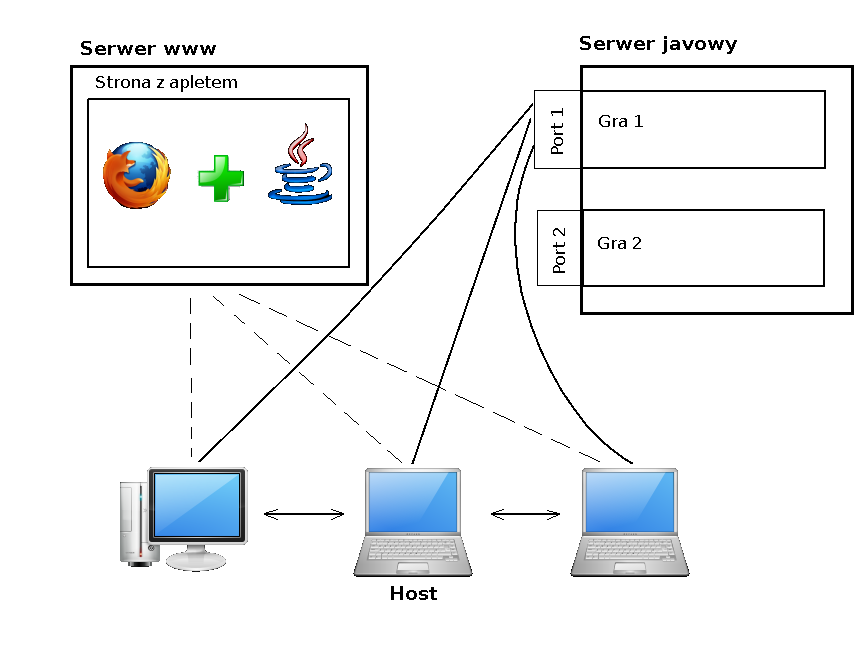
\includegraphics[scale=0.6]{rysunki/arch.png}
\caption{Schemat architektury}
\label{fig:arch}
\end{figure}

\subsection{Rozgrywka}
Rozgrywka może znajdować się w jednym z trzech stanów:
\begin{enumerate}
 \item \textbf{Nierozpoczęta.} W tym stanie do rozgrywki mogą dołączać gracze. Nazwa rozgrywki jest widoczna w aplikacjach klientów znajdujących się w trybie menu (Rysunek~\ref{fig:menu}). Gospodarz rozgrywki może ustawiać parametry związane z grą (Rysunek~\ref{fig:inicjacja}). 

 \item \textbf{Rozpoczęta.} Nazwa rozgrywki znika z listy widocznej na Rysunku~\ref{fig:menu}, użytkownicy tracą możliwość dołącznia do niej. Gospodarz otrzymuje od serwera gniazda do gości, a goście gniazdo do gospodarza. Na komputerze gospodarza inicjowane są wszystkie obiekty związane z grą i rozgrywka się rozpoczyna.

 \item \textbf{Zakończona.} Rozgrywka się zakończyła, lecz gospodarz jeszcze jej nie opuścił.
\end{enumerate}

\subsection{Tryby klienta}
Aplikacja klienta w każdym momencie znajduje się w jednym z trzech trybów.

\paragraph{Tryb menu.} Jest to tryb ``międzyrozgrywkowy''.

\begin{figure}
\centering
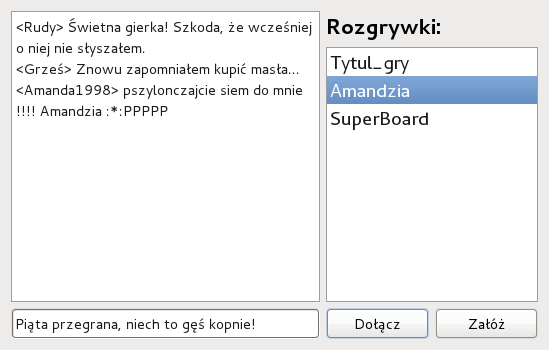
\includegraphics[scale=0.8]{rysunki/menu.png}
\caption{Aplikacja w trybie menu.}
\label{fig:menu}
\end{figure}

Aplikacja prezentuje swojemu użytkownikowi rozgrywki, do których może się przyłączyć, daje możliwość rozpoczęcia nowej rozgrywki oraz porozmawiania z pozostałymi graczami na czacie. Przedstawia to Rysunek~\ref{fig:menu}. Jeśli użytkownik postanowi zostać gospodarzem nowej rozgrywki wyświetli mu się okienko dialogowe przedstawione na Rysunku~ \ref{fig:nowagra}. Użytkownik nadaję rozgrywce nazwę, która zostanie zaprezentowana pozostałym graczom. Rozgrywka może być publiczna -- wtedy każdy użytkownik może do niej dołączyć, lub prywatna, wtedy należy podać hasło pozwalające na dołączenie do rozgrywki. 

\begin{figure}
\centering
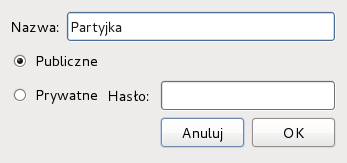
\includegraphics[scale=0.8]{rysunki/nowagra.png}
\caption{Rozpoczynanie nowej rozgrywki.}
\label{fig:nowagra}
\end{figure}

\paragraph{Tryb hosta.} W tym trybie klient staje się gospodarzem rozgrywki. Początkowo oczekuje aż dołączy odpowiednio wielu graczy. Użytkownicy, których klienty znajdują się w trybie menu, widzą tę rozgrywkę na swoim panelu i mogą do niej dołączyć. W tym czasie gospodarz może ustawić parametry związane z grą, co przedstawia Rysunek~\ref{fig:inicjacja}.

\begin{figure}
\centering
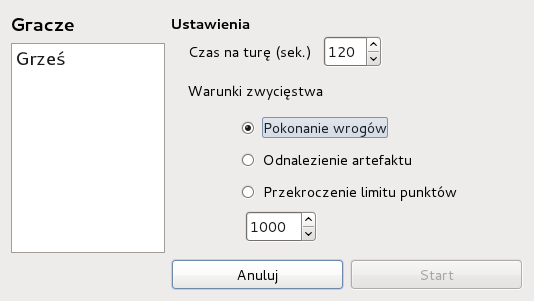
\includegraphics[scale=0.8]{rysunki/inicjacja.png}
\caption{Przykładowy panel gospodarza przed rozpoczęciem rozgrywki.}
\label{fig:inicjacja}
\end{figure}

Po pojawieniu się wymaganej liczby graczy rozgrywka może zostać rozpoczęta. Znika wówczas z listy dostępnych rozgrywek. Aplikacja gospodarza odpowiada za wykonywanie wszelkich obliczeń i operacji związanych z grą. Wszystkich gości informuje tylko o zmianach stanów istotnych obiektów, tak aby aplikacje gości mogły je należycie wyświetlić swoim użytkownikom. Goście przekazują swoje ruchy gospodarzowi, który uwzględnia je w logice gry. Ponadto aplikacja w trybie hosta wykonuje te same zadania, co aplikacja w trybie gościa, ponieważ jej użytkownik także jest graczem.

\paragraph{Tryb gościa.} W tym trybie aplikacja służy do wyświetlania stanu gry swojemu użytkownikowi oraz przekazywania jego ruchów gospodarzowi rozgrywki.

\subsection{Wątki serwera.}
Hierarchię wątków przedstawia Rysunek~\ref{fig:watki}.

\begin{figure}
\centering
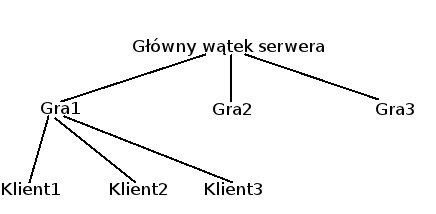
\includegraphics{rysunki/watki.png}
\caption{Wątki serwera.}
\label{fig:watki}
\end{figure}

Główny wątek serwera udostępnia panel administracyjny, przy pomocy którego można dodawać nowe gry, albo usuwać je, jeżeli nie cieszą się zainteresowaniem, blokować użytkowników jeżeli szkodzą oni innym, na przykład nadużywając wulgaryzmów na czacie, itp.

Dodanie nowej gry tworzy nowy wątek. Odpowiada on za nasłuchiwanie na przeznaczonym dla niego porcie. Po nawiązaniu połącznia z klientem tworzony jest wątek dla tego klienta.

Wątek klienta odpowiada za komunikację z nim. Została ona opisana w sekcji~\ref{sec:komunikacja}.

\subsection{Zadania elementów systemu}
\paragraph{Serwer www.}
Strona internetowa w elegancki sposób przedstawia ofertę gier. Służy lokalnym maszynom do ``pobrania'' apletu.

\paragraph{Serwer dedykowany.}
Dla każdej gry tworzy odzielny wątek do obsługi tej gry, który:
\begin{itemize}
 \item przechowuje listę gniazd klientów,
 \item rozpropagowuje wiadomości wysłane na czacie,
 \item pośredniczy w rozpoczęciu rozgrywki przez graczy.
\end{itemize}

\paragraph{Aplet.}
\begin{enumerate}
 \item W trybie menu:
    \begin{itemize}
      \item umożliwia komunikację użytkowników poprzez czata,
      \item przedstawia listę nierozpoczętych rozgrywek,
      \item daje możliwość dołączenia do nierozpoczętej rozgrywki lub założenia nowej.
    \end{itemize}

 \item W trybie hosta:
    \begin{itemize}
      \item służy ustawieniu parametrów rozgrywki i jej rozpoczęciu,
      \item odpowiada za uaktualnianie logiki rozgrywki,
      \item przyjmuje od gości informacje o ich ruchach,
      \item wysyła gościom informacje o aktualnym stanie rozgrywki,
      \item pełni także takie funkcje jak klienty w trybie gościa, ponieważ gospodarz także jest graczem.
    \end{itemize}

 \item W trybie gościa:
    \begin{itemize}
      \item przyjmuje od gospodarza komunikaty o aktualnym stanie rozgrywki,
      \item wyświetla użytkownikowi stan rozgrywki (na przykład w przypadku szachów będzie do rysunek szachownicy i bierek),
      \item oczekuje na ruchy swojego użytkownika (w przypadku szachów kliknięcia na bierki i pola), a następnie wysła je gospodarzowi.
    \end{itemize}
\end{enumerate}

\section{Dane przechowywane przez elementy systemu}
\begin{Large}
\textcolor{red}{Do poprawienia!}
\end{Large}
\subsection{Klient}
Niezależnie do trybu klient ma w pamięci gniazdo umożliwiające komunikację z serwerem.
Ponadto w trybie: 
  \begin{itemize}
   \item \textbf{hosta} - przechowuje gniazda służące do kontaktu z klientami-gośćmi. Posiada wszystkie obiekty związane z rozgrywką. 
   \item \textbf{gościa} - przechowuje gniazdo przeznaczone do komunikacji z gospodarzem.
  \end{itemize}
\subsection{Serwer}
Wątek gry przechowuje:
\begin{itemize}
 \item listę wszystkich połączonych klientów i ich pseudonimy,
 \item listę wszystkich rozgrywek,
 \item listę wszystkich wolnych klientów (będących w trybie menu),
 \item listę zajętych klientów wraz z referencjami do rozgrywki, w której biorą udział.
\end{itemize}


\section{Komunikacja między serwerem i klientami}
\label{sec:komunikacja}

\subsection{Komunikaty z serwera do klienta}
\begin{center}
 \begin{tabular}{p{1.3cm}||p{5.2cm}||p{7cm}}
 \hbox{Tryb} klienta& Rodzaj komunikatu & Co powinien zrobić klient?\\ \hline \hline
\multirow{8}{*}{Menu}
  & wiadomość na czacie
  & Wyświetlić ją w okienku czata. \\ \cline{2-3}

  & lista wszystkich dostępnych rozgrywek
  & Wypisać je na przeznaczonej do tego liście. \\ \cline{2-3}

  & informacja o nowej rozgrywce
  & Dopisać do listy dostępnych rozgrywek. \\ \cline{2-3}

  & informacja o nieaktualności pewnej rozgrywki\footnotemark
  & Usunąć z listy dostępnych rozgrywek. \\ \cline{2-3}

  & akceptacja utworzenia nowej rozgrywki
  & Przełączenie się w tryb hosta. \\ \cline{2-3}

  & odrzucenie nowej rozgrywki\footnotemark
  & Wyświetlić komunikat z przyczyną. \\ \cline{2-3}

  & akceptacja dołączenia do rozgrywki 
  & Przejście w tryb gościa. \\ \cline{2-3}

  & odrzucenie prośby o dołącznie do rozgrywki\footnotemark
  & Wyświetlić ją w stosownym okienku. \\ \hline \hline

\multirow{2}{*}{Host}
  & dołączenie gracza
  & Sprawdzić czy można rozpocząć rozgrywkę. \\ \cline{2-3}

  & odejście gracza
  & Jeżeli rozgrywka nie jest rozpoczęta, to być może należy wyłączyć możliwość rozpoczęcia gry. Jeżeli jest rozpoczęta, to postępownaie zależy od konkretnej gry. \\ \hline \hline

  Gość
  & odejście gospodarza
  & Wyświetlić komunikat o przerwaniu gry i wrócić do trybu gościa. \\ \hline \hline
\end{tabular}
\end{center}

\footnotetext[1]{Przyczyną tego może być osiągnięcie maksymalnej liczby graczy, rezygnacja gospodarza, rozpoczęcie rozgrywki.}
\footnotetext[2]{Z powodu nieprawidłowej nazwy rozgrywki - już istniejącej, zawierającej niedozwolne znaki, pustej, etc.}
\footnotetext[3]{Nieprawidłowe hasło lub rozgrywka zapełniona (może się to zdarzyć jeśli dwóch graczy w tym samym momencie spróbuje dołączyć do gry, której brakuje jednego gracza).}

Dodajmy jeszcze, że kiedy klient dołącza do gry serwer przekazuje mu gniazdo do komunikacji z hostem, a hostowi gniazdo do komunikacji z klientem. 

\subsection{Komunikaty od klienta do serwera}

\begin{center}
 \begin{tabular}{p{1.3cm}||p{3.5cm}||p{9cm}}
 \hbox{Tryb} klienta& Rodzaj komunikatu & Co powinien zrobić serwer?\\ \hline \hline
\multirow{3}{*}{Menu}
  & wiadomość na czacie
  & Rozpropagować wśród wszystkich wolnych klientów (tzn. będących w trybie menu). \\ \cline{2-3}

  & rozpoczęcie nowej rozgrywki
  & Jeżeli nazwa gry jest poprawna\footnotemark, to:
      \begin{itemize}
      \item poinformować klienta o akceptacji rozgrywki,
      \item przesłać pozostałym klientom komunikat o nowej rozgrywce,
      \item utworzyć obiekt rozgrywki,
      \item przepisać klienta z listy wolnych do zajętych z referencją do utworzonej rozgrywki.
      \end{itemize}
    W przeciwnym razie wysłać klientowi komunikat o odrzuceniu rozgrywki. \\ \cline{2-3}

  & prośba o dołączenie do rozgrywki,
  & Jeżeli z jakiegoś powodu klient nie może do niej dołączyć, to wysyłamy stosowny komunikat. W przeciwnym razie przepisujemy klienta z listy wolnych do zajętych z referencją do odpowiedniej rozgrywki.\\ \hline
\end{tabular}
\end{center}

\footnotetext{Patrz przypis [2].}

\begin{center}
 \begin{tabular}{p{1.3cm}||p{3.5cm}||p{9cm}}
\hline
\multirow{2}{*}{Host}
  & odejście z rozgrywki
  & Wszystkim gościom wysyłamy komunikat o odejściu gospodarza. Przepisujemy wszystkich z listy zajętych do wolnych i usuwamy obiekt rozgrywki.\\ \cline{2-3}

  & rozpoczęcie rozgrywki
  & Informujemy wolnych klientów, że rozgrywka jest już nieaktualna.\\ \hline \hline

Guest & odejście z rozgrywki & Usuwamy klienta z list zajętych i umieszczamy na liście wolnych. Wysyłamy gospodarzowi rozgrywki komunikat o odejściu gościa.

\end{tabular}
\end{center}


\subsection{Komunikacja gość-gospodarz}
Komunikacja między gospodarzem i jego gośćmi może być dowolnie zdefiniowana przez programistę gry.

Odnotujmy jedynie, że w systuacji, gdy któraś ze stron odchodzi z gry, to informowany jest serwer, a nie klienci. Robimy tak dlatego, że w przypadku zerwania połącznia klient nie powiadomi innych o swoim odejściu. Ten obowiązek i tak spocznie na serwerze. Dlatego przyjmujemy, że o odejściu gracza zawsze informuje serwer, nawet gdy odbywa się ono poprzez wybranie odpowiedniej opcji w menu.

\subsection{Zerwanie połączenia}
W przypadku, gdy połączenie z klientem zostanie przerwane serwer musi podjąć pewne działania. Jeśli klient znajdował się w trybie:
\begin{itemize}
 \item \textbf{hosta} - powiadamiamy wszystkich gości w rozgrywce o jego odejściu i usuwamy rozgrywkę.
 \item \textbf{gościa} - powiadamiamy hosta o odejściu klienta.
\end{itemize}
 Niezależnie od trybu w jakim znajdował się klient, należy go usunąć ze wszystkich list na jakich się znajduje i zakończyć wątek przeznaczony do jego obsługi.

\section{Hierarchia klas}
TODO!!!

\section{Słownik}
\begin{description}
 \item[Gra] - rodzaj zabawy towarzyskiej, u nas internetowej, odbywający się według określonych reguł, na przykład: szachy, chińczyk.
 \item[Rozgrywka] - jest to przebieg pewnej gry, na przykład: partia szachów.
 \item[Gospodarz, Host] - klient, na którego komputerze odbywa się logika rozgrywki.
 \item[Gość] - klient biorący udział w rozgrywce, niebędący gospodarzem.
 \item[Logika rozgrywki] - stan rozgrywki, wartości wszystkich obiektów związanych z rozgrywką.
\end{description}

\end{document} 
